\documentclass{article}
%% Useful packages
\usepackage[utf8]{inputenc}
\usepackage{float}
\usepackage[final]{graphicx}
\usepackage[a4paper,left=2cm,right=2cm,top=2cm,bottom=2cm]{geometry}
\usepackage{crop,graphicx,amsmath,array,color,amssymb,fancyhdr,lineno}
\usepackage{flushend,stfloats,amsthm,chngpage,times,,lipsum,lastpage}
\usepackage{calc,listings,color,wrapfig,tabularx,longtable,enumitem}
\usepackage[style=numeric-comp,backend=biber]{biblatex}
\usepackage[utf8]{inputenc}
\usepackage{pgfplots}
\usepackage{multicol}
\pgfplotsset{width=10cm,compat=1.9}
\usepgfplotslibrary{external}
\usepgfplotslibrary{dateplot}
\tikzexternalize
\addbibresource{Refs.bib}
\usepackage{lineno}
%%%%%%%%%%%%   Header and Footer  %%%%%%%%%%%%%
\pagestyle{fancy}
\fancypagestyle{plain}{%
  \renewcommand{\headrulewidth}{0pt}%
  \fancyhf{}%
}

\title{%
  Lab 2\\
  \large MapReduce with Hadoop on AWS}
\author{Random Name}

\begin{document}
\begin{titlepage}

\newcommand{\HRule}{\rule{\linewidth}{0.5mm}} % Defines a new command for the horizontal lines, change thickness here

%----------------------------------------------------------------------------------------
%	LOGO SECTION
%----------------------------------------------------------------------------------------
\center

\includegraphics[width=10cm]{Title/polytechnique.png}\\[1cm] % Include a department/university logo - this will require the graphicx package
 
%----------------------------------------------------------------------------------------

\center % Center everything on the page

%----------------------------------------------------------------------------------------
%	HEADING SECTIONS
%----------------------------------------------------------------------------------------

\textsc{\LARGE Polytechnique Montréal }\\[1.5cm] % Name of your university/college
\textsc{\Large LOG8415E}\\[0.5cm] % Major heading such as course name
\textsc{\large Advanced Concepts of Cloud Computing}\\[0.5cm] % Minor heading such as course title

%----------------------------------------------------------------------------------------
%	TITLE SECTION
%----------------------------------------------------------------------------------------
\makeatletter
\HRule \\[0.4cm]
{ \huge \bfseries \@title}\\[0.4cm] % Title of your document
\HRule \\[1.5cm]
 
%----------------------------------------------------------------------------------------
%	AUTHOR SECTION
%----------------------------------------------------------------------------------------

\begin{minipage}{0.4\textwidth}
\begin{flushleft} \large
\emph{Authors:}\\
2009913 - Jordan Mimeault\\
2018968 - Antoine Lombardo\\
2020511 - Jacob Dupuis\\
2024785 - Alexandre Dufort\\[1.2em]
\end{flushleft}
\end{minipage}
~
\begin{minipage}{0.4\textwidth}
\begin{flushright} \large
\emph{Lab Instructor:} \\
Vahid Majdinasab  \\[1.2em] % Supervisor's Name
\emph{Instructor:} \\
Amin Nikanjam % second marker's name
\end{flushright}
\end{minipage}\\[2cm]
\makeatother

% If you don't want a supervisor, uncomment the two lines below and remove the section above
%\Large \emph{Author:}\\
%John \textsc{Smith}\\[3cm] % Your name

%----------------------------------------------------------------------------------------
%	DATE SECTION
%----------------------------------------------------------------------------------------

{\large October 17, 2022}\\[2cm] % Date, change the \today to a set date if you want to be precise

\vfill % Fill the rest of the page with whitespace

\end{titlepage}

\sffamily

\fancyhf{}
\fancyhead[L]{LOG8415E}
\fancyhead[R]{Lab 2}
\fancyfoot[R]{ \bf\thepage\ \rm }%

\newpage
\tableofcontents

\newpage
\section{Experiments with WordCount program.} \label{T1}

\paragraph{}To wrap all WordCount implementations, we decided to create a Docker image that expose a REST API allowing us to send WordCount tasks to any desired implementation. This Docker image is available on Docker Hub (`lombardoa/tp2`) and can be run locally or on a AWS Instance. 

\paragraph{}Running the image locally is straight forward. Deploying the image on a AWS instance can be automatically done using our script and will be shown in the last section of this document.

\paragraph{}We started by creating a Docker image based on Ubuntu 20.04. We then installed Java and Hadoop and did the configuration for Hadoop to run in standalone mode. We then copied the input file `pg4300.txt`. After testing it by passing through the instance shell, we then created a Flask wrapper that run Hadoop MapReduce task using the linux `time` command, wait for the completion and read and process the output of both Hadoop and time. By doing so, we can use the REST API to start MapReduce task and receive its execution time and its output as a response. We used this interface to do the performance comparisons of the next section.

\paragraph{}For the Linux WordCount program, we simply created a bash script that splits the content of the input file in words by using the `tr` command, then sort these words by using the `sort` command, then count the occurence of each words using the `uniq -c` command. The script output its result in the stdout stream. We then added a Flask route for running a WordCount using this script, again using the `time` command.

\paragraph{}Finally, implementing Spark WordCount was straigth forward, since there are multiple guides online explaining how to do it. We then created a Python script that execute a WordCount program using Spark, then once again wrapped it inside our Flask app.

\paragraph{}This gives us three different routes that we used in the next section to create a benchmark script:

\begin{itemize}
  \item http://\{address\}/hadoop/wordcount/\{input\_file\}
  \item http://\{address\}/spark/wordcount/\{input\_file\}
  \item http://\{address\}/linux/wordcount/\{input\_file\}
\end{itemize}
\pagebreak













\section{Performance comparison of Hadoop vs. Linux} \label{T2}

\paragraph{}We created two clusters (target groups) named cluster1 and cluster2. cluster1 targets every t2 instances, while cluster2 targets every m4 instances. These target groups allows us to redirect traffic to the desired type of instance, depending on the rules specified in the Load Balancer.
\paragraph{}For the Load Balancer, we created an internet-facing Application Load Balancer. We then added a Listener that listens to the HTTP port 80. We specified rules to redirect traffic to the correct clusters, depending on the path that needs to be accessed. The first rule forwards the request to cluster1 if the path is /cluster1, the second rule forwards the request to cluster2 if the path is /cluster2, and the default route returns a fixed response which is a 404 NOT FOUND error, indicating that the routes leads to no specified cluster.


\pagebreak
\section{Performance comparison of Hadoop vs. Spark on AWS.} \label{T3}
\paragraph{}To perform this comparison, we run the WordCount script 3 times on each file for both Hadoop and Spark to get an approximate average run-time for each file. Again, these tests were made on the AWS Instance, but have also been done locally to confirm their validity. Here is a graph comparing Hadoop and Spark performances.\\
\begin{center}
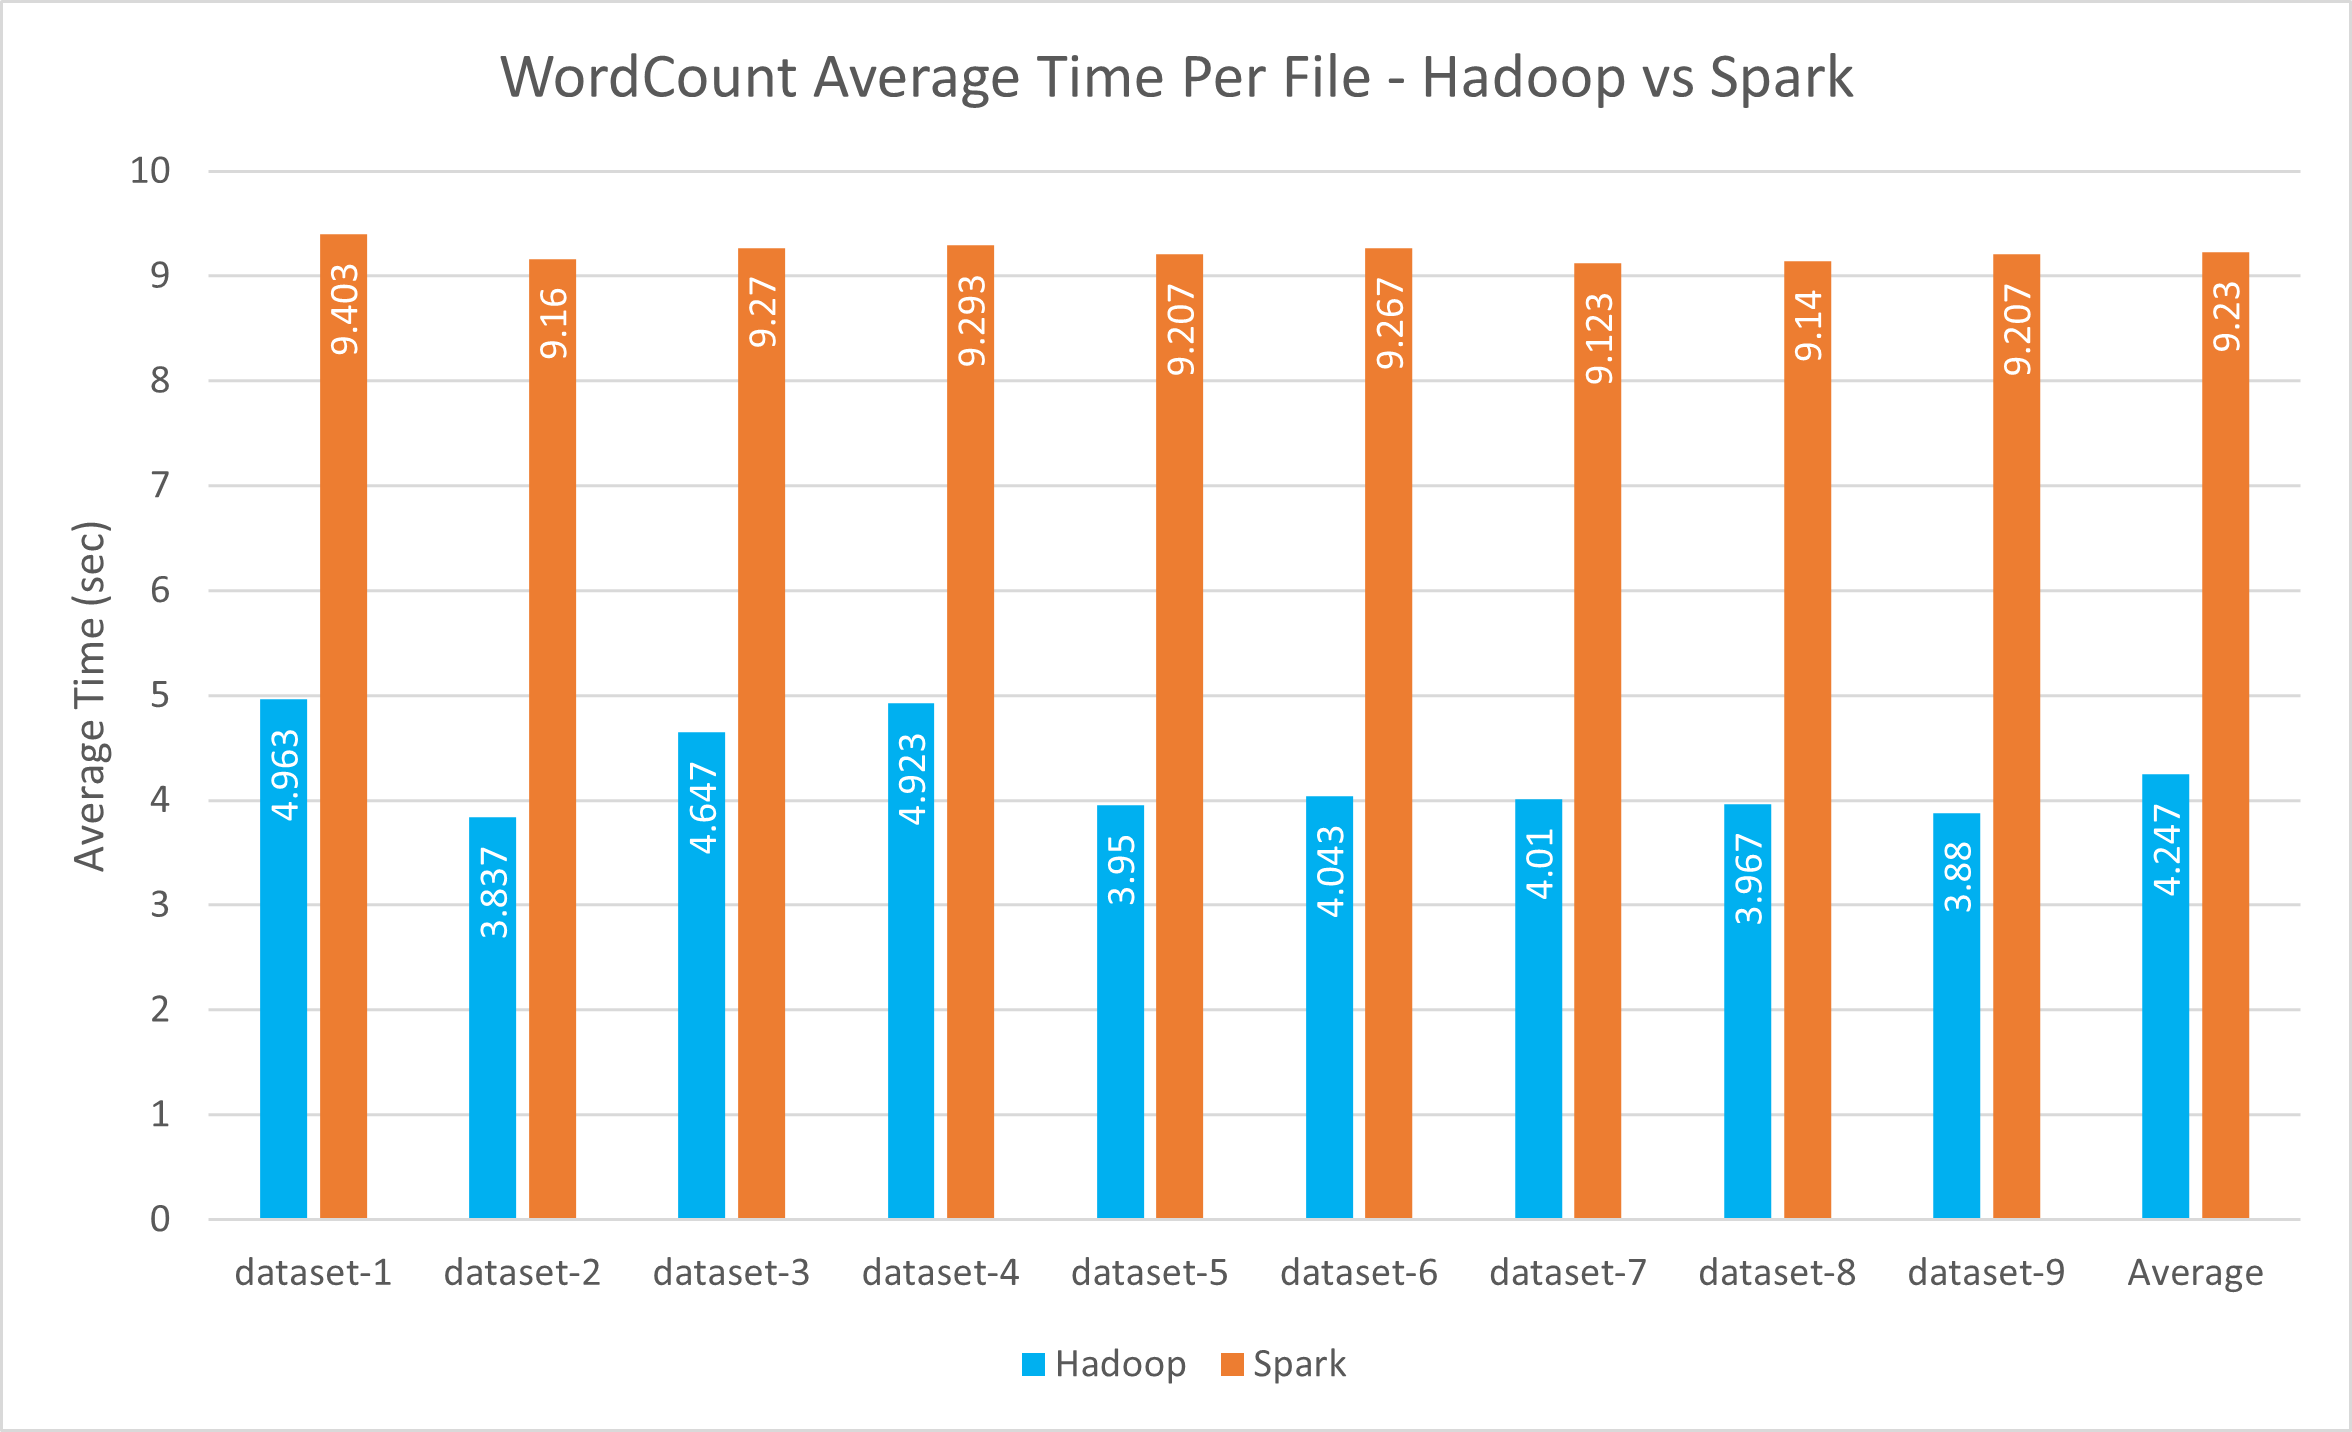
\includegraphics[width=14cm]{Resources/hadoop_vs_spark.png}\\
\emph{Figure 3.1 - Hadoop vs Spark average time}
\end{center}
\paragraph{}From the above graph, we can conclude that Hadoop is about 2 times faster than Spark. This is in contradiction with what we tought would happen, as Spark is known to be able to run up to 100 times faster than Hadoop. This once again can be explained by the fact that Spark has to load the dataset in memory and make connections between everything it has loaded in memory, which are two very expensive operations. With a very large dataset, this step would have a minimal impact over the whole task, but since our dataset is very small, these two steps have a large impact on the results.
\pagebreak
\section{Describe how you have used MapReduce jobs to solve the social network problem.} \label{T4}

\paragraph{}The script needs to be run and should run correctly on any linux environment. However, it has only been tested on a Debian environment. The pre-requisite to run the script is to have git, pip3, python3, aws and docker installed. To make sure the script is executable, the command \verb|sudo chmod +x script.sh| must be executed. Our bash script can then be run as root with the command \verb|sudo .\script.sh|. Out git repository will then be automatically cloned and the \verb|run.sh| script will be executed, which will automatically install all the necessary Python libraries.

\paragraph{}Alternatively, the script can be run manually. To do so, the repository must be cloned using this command:\\\verb|git clone https://github.com/JordMim/LOG8415E.git|. The script will then be located in the directory \verb|LOG8415E/tp1|. The script must be set as executable using the command \verb|sudo chmod +x run.sh|, and can then be run using the command \verb|sudo ./run.sh|.

\paragraph{}When running the script, you'll be asked to setup AWS credentials. If this is your first time using the script, you'll have to do this setup. After that, this step can be omitted, as it will fetch the default credentials saved in AWS.\\




\paragraph{}When AWS configuration is done, you'll be asked what actions needs to be done. There are five options:
\begin{itemize}
  \item Configure AWS Load Balancer, which basically creates all the necessary AWS resources.
  \item Run requests sender, which runs the benchmark.
  \item Fetch metrics, which fetch CloudWatch metrics and export them into JSON and latex format.
  \item Only run benchmark and fetch metrics.
  \item Do everything.
\end{itemize}






\section{Describe your algorithm to tackle the social network problem.} \label{T5}

\paragraph{}To solve the social network problem we had to use the map reduce algorithm to treat the data. Initially, we had every user id and their list of friends. The goal is to recommend to the user a list of mutual friend between himself and his friends. 

\paragraph{}To approach this problem, we created a Recommendation class that has two attributes: a int representing the friend to add as a recommendation and another int representing the mutual friend. The mutual friend field has a value of -1 if he is a direct friend of the current user. 

\paragraph{}For the Map function, it process a text line to retrieve the user and his list of friend. From the moment that a user has friends, for each friend we add him to the list of friends of the user. Then, we write with the user as the key and a recommendation of the friend with a mutual friend value of -1 as the value, the format is as followed : Recommendation(friend, -1). This indicates that this direct friend can be omitted in the reduce step. After all friends are added to the friends list, we wrote recommendations in both ways for each pair of friend, because they all have the current user as mutual.

\paragraph{}For the Reduce function, we start by counting all the recommended users that have the same key and that are not direct friend (!= -1) by merging the same keys in an HashMap. Then, we used a comparator to sort our map by reverse key and then by value. After filtering the entries by removing the recommended users already friends with the user, we kept the 10 most recommended friends and added them to a final recommendation list of friend. The final step was to write this final recommendation as the values and the user as the key in the format of the initial text file.
\pagebreak
\section{Recommendations of connection for the users} \label{T6}

\paragraph{}This is our recommendation for the user with following user IDs: 924, 8941, 8942,
9019, 9020, 9021, 9022, 9990, 9992, 9993.\\
\begin{description}
  \item[$\bullet$ 924: ] 439, 2409, 6995, 11860, 15416, 43748, 45881
  \item[$\bullet$ 8941: ] 8943,
        8944,
        8940
  \item[$\bullet$ 8942: ]8939,
        8940,
        8943,
        8944
  \item[$\bullet$ 9019: ] 022,
        317,
        9023
  \item[$\bullet$ 9020: ]  9021,
        9016,
        9017,
        9022,
        317,
        9023
  \item[$\bullet$ 9021: ] 9020,
        9016,
        9017,
        9022,
        317,
        9023
  \item[$\bullet$ 9022: ] 9019,
        9020,
        9021,
        317,
        9016,
        9017,
        9023
  \item[$\bullet$ 9990: ] 13134,
        13478,
        13877,
        34299,
        34485,
        34642,
        37941
  \item[$\bullet$ 9992: ] 9987,
        9989,
        35667,
        9991
  \item[$\bullet$ 9993: ] 9991,
        13134,
        13478,
        13877,
        34299,
        34485,
        34642,
        37941
\end{description}
\paragraph{}The list of all filtered Ids (\emph{output-report.json}) and the list of all Ids (\emph{output-all.json}) can be found in the \emph{tp2/social-network-client}  directory \\
\section{Summary of results and instructions to run your code.} \label{T7}

\paragraph{}To conclude, the above results shows us that both Hadoop and Spark gives no advantages when working with small datasets. However, if our datasets were a lot larger and the problem more complex, using Hadoop or Spark could have a significant performance impact over a plain Linux solution.

\paragraph{}The script needs to be run and should run correctly on any linux environment. However, it has only been tested on a Debian environment. To run our code, Python 3, Pip 3, Git and AWS CLI have to be installed on your machine. To make sure the script is executable, the command \verb|sudo chmod +x script.sh| must be executed. Our bash script can then be run as root with the command \verb|sudo ./script.sh|. Out git repository will then be automatically cloned and the \verb|run.sh| script will be executed, which will launch an interactive dialog.

\paragraph{}Alternatively, the script can be run manually. To do so, the repository must be cloned using this command:\\\verb|git clone https://github.com/JordMim/LOG8415E.git|. The script will then be located in the directory \verb|LOG8415E/tp2|. The script must be set as executable using the command \verb|sudo chmod +x run.sh|, and can then be run using the command \verb|sudo ./run.sh|.

\paragraph{}The deployment of our application on an AWS instance can be done using the first option of our run.sh script. This script guides the user while configuring AWS, then run a Python script that uses Boto3 for creating and configuring the Security Group and the Instance.

\paragraph{}To simplify the deployment on our AWS Instance, we decided to create a Docker image on which every dependencies are installed. By user a user\_data script, we automatically install Docker on the Instance and run a container based on this Docker image. This Docker image is based on Ubuntu 20.04 and contains Java 11, Hadoop 3.3.4, Python 3, PySpark 3.3.1. It also contain all the datasets. This all-in-one image gives the user the access over all the functionality through a REST API that respond to the port 80.

\paragraph{}More infos on the usage of the script is provided in the \href{https://github.com/JordMim/LOG8415E/blob/main/tp2/README.md}{\textbf{\emph{README.md}}} file of our repository.

\paragraph{}For each step of the script, the normal output should look like these:

\begin{center}
    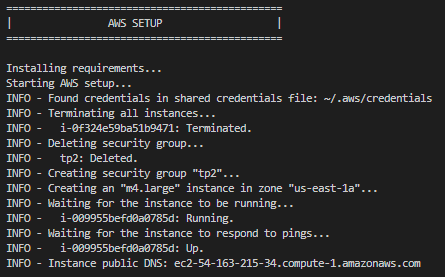
\includegraphics[width=14cm]{Resources/setup.png}\\
    \emph{Figure 7.1 - Output of the AWS Setup step}\\
    \hfill\\
    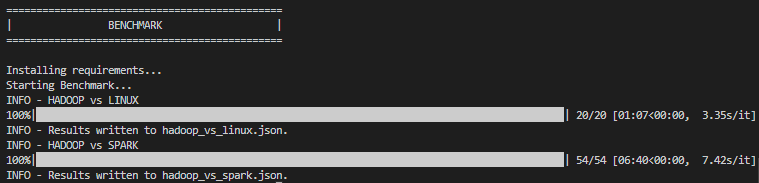
\includegraphics[width=14cm]{Resources/benchmark.png}\\
    \emph{Figure 7.2 - Output of the Benchmark step}\\
    \hfill\\
    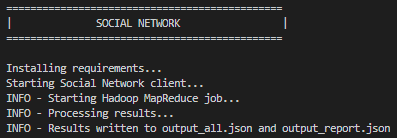
\includegraphics[width=14cm]{Resources/social.png}\\
    \emph{Figure 7.3 - Output of the Social Network step}\\
\end{center}


\pagebreak
\printbibliography[heading=bibnumbered]


\end{document}
